% $Id$
%\documentclass[handout]{beamer}
\documentclass{beamer}
\usepackage[utf8]{inputenc}
\usepackage[T1]{fontenc}
\usepackage[english,swedish]{babel}
\usepackage{url}
\usepackage{graphicx}
\usepackage{color}
\usepackage{subfig}
\usepackage{multicol}
\usepackage{amssymb,amsmath,amsthm}
\usepackage{booktabs}
\usepackage[squaren,binary]{SIunits}
\usepackage{verbatim}

\usepackage{algpseudocode}
\newenvironment{algorithm}[1]{%
  \begin{block}{Algorithm (#1)}
}{%
  \end{block}
}

\setbeamertemplate{bibliography item}[text]
\usepackage[natbib,style=alphabetic,maxbibnames=99]{biblatex}
\addbibresource{pubkey.bib}

%\newtheorem{theorem}{Sats}%[chapter]
%\newtheorem{lemma}{Lemma}
%\newtheorem{corollary}{Korollarium}
\theoremstyle{definition}
%\newtheorem{definition}{Definition}
%\newtheorem{axiom}[definition]{Axiom}
%\newtheorem{example}{Exempel}
\newtheorem{exercise}{Övning}

\DeclareMathOperator{\p}{\mathcal{P}}
\let\P\p
\DeclareMathOperator{\C}{\mathcal{C}}
\DeclareMathOperator{\K}{\mathcal{K}}
\DeclareMathOperator{\E}{\mathcal{E}}
\DeclareMathOperator{\D}{\mathcal{D}}
\DeclareMathOperator{\X}{\mathcal{X}}
\DeclareMathOperator{\Y}{\mathcal{Y}}
\DeclareMathOperator{\h}{\mathcal{H}}
\let\H\h

\DeclareMathOperator{\N}{\mathbb{N}}
\DeclareMathOperator{\Z}{\mathbb{Z}}
\DeclareMathOperator{\R}{\mathbb{R}}

\let\stoch\mathbf

\renewcommand{\p}{\stoch P}
\renewcommand{\c}{\stoch C}
\renewcommand{\k}{\stoch K}
\newcommand{\x}{\stoch X}
\newcommand{\y}{\stoch Y}
\newcommand{\e}{\stoch E}
\newcommand{\s}{\stoch S}

\DeclareMathOperator{\lequiv}{\Longleftrightarrow}
\DeclareMathOperator{\xor}{\oplus}

\renewcommand{\qedsymbol}{Q.E.D.}

\DeclareMathOperator{\hmac}{HMAC}
\DeclareMathOperator{\concat}{||}

\mode<presentation>
{
  \usetheme{Frankfurt}
  \setbeamercovered{transparent}
  \usecolortheme{seagull}
}
\setbeamertemplate{footline}{\insertframenumber}

% XXX translate pubkey lecture to English
\title{%
  Asymmetrisk kryptografi och meddelandeautentisering
}
\author{Daniel Bosk\footnote{%
  Detta verk är tillgängliggjort under licensen Creative Commons 
  Erkännande-DelaLika 2.5 Sverige (CC BY-SA 2.5 SE).
	För att se en sammanfattning och kopia av licenstexten besök URL 
	\url{http://creativecommons.org/licenses/by-sa/2.5/se/}.
}}
\institute[MIUN IKS]{%
  %Department of Information and Communication Systems (ICS),\\
  %Mid Sweden University, Sundsvall.
  Avdelningen för informations- och kommunikationssytem (IKS),\\
  Mittuniversitetet, SE-851\,70 Sundsvall.
}
\date{\today}

%\pgfdeclareimage[height=0.65cm]{university-logo}{MU_logotyp_int_CMYK.pdf}
%\logo{\pgfuseimage{university-logo}}

\AtBeginSection[]{%
  \begin{frame}<beamer>{Översikt}
    \small
    \tableofcontents[currentsection]
  \end{frame}
}

\begin{document}

\begin{frame}
  \titlepage
\end{frame}

\begin{frame}{Översikt}
  \tableofcontents
\end{frame}


% Since this a solution template for a generic talk, very little can
% be said about how it should be structured. However, the talk length
% of between 15min and 45min and the theme suggest that you stick to
% the following rules:  

% - Exactly two or three sections (other than the summary).
% - At *most* three subsections per section.
% - Talk about 30s to 2min per frame. So there should be between about
%   15 and 30 frames, all told.


% XXX add slides about key management

\section{Asymmetrisk kryptografi}

\subsection{Introduktion}

\begin{frame}{\insertsubsectionhead}
  \begin{figure}
    \includegraphics[height=0.7\textheight]{asymmetric.eps}
    \caption{Översikt av asymmetrisk kryptering.
      Bild: \cite{Stallings2011can}.}
  \end{figure}
\end{frame}

\begin{frame}{\insertsubsectionhead}
  \begin{theorem}[Fermat--Eulers sats]
    \begin{enumerate}
      \item Om \(n\) och \(a\) är heltal sådana att \(\gcd(n, a) = 1\),
      \item då gäller att \(a^{\phi(n)}\equiv 1\pmod n\),
      \item[] där \(\phi(n) = p_1^{e_1-1}(p_1-1)\cdots p_m^{e_m-1}(p_m-1)\),
      \item[] \(p_i\) är alla primtalsfaktorer och \(e_i\) respektive exponent 
        för \(n = p_1^{e_1} p_2^{e_2}\cdots p_m^{e_m}\).
    \end{enumerate}
  \end{theorem}
  \begin{example}
    \begin{enumerate}
      \item Låt \(n = 10\) och \(a = 3\) (\(a\) får inte vara på formen \(a = 
        2k\) eller \(a = 5k\) för \(k\in \N\)).
        Då är \(\gcd(n, a) = \gcd(10, 3) = 1\).
      \item Vi har också \(a^{\phi(n)}\equiv 3^{(2-1)(5-1)}\equiv 3^4\equiv 
        81\equiv 1\pmod n.\)
    \end{enumerate}
  \end{example}
\end{frame}

%\begin{frame}{\insertsubsectionhead}
%  \begin{proof}[Bevis för Fermat--Eulers sats]
%    \dots
%  \end{proof}
%\end{frame}

\subsection{Kryptosystem}

\begin{frame}{\insertsubsectionhead}{Rivest, Shamir, Adleman (RSA)}
  \begin{definition}
    Låt \(n = pq\), där \(p\) och \(q\) är primtal.
    Låt \(\P = \C = \Z_n\) och
    \begin{align*}
      \K = \{ (n, p, q, e, d)\colon ed\equiv 1\pmod{\phi(n)}\}.
    \end{align*}
    För \(k = (n, p, q, e, d)\) definiera
    \begin{align*}
      e_k(p) &= p^e\mod n \text{ och} \\
      d_k(c) &= c^d\mod n,
    \end{align*}
    där \(p\in \P\) och \(c\in \C\).
    Tupeln \((n, e)\) utgör den \emph{publika nyckeln} och \((p, q, d)\) den 
    \emph{privata nyckeln}.
  \end{definition}
\end{frame}

\begin{frame}{\insertsubsectionhead}
  \begin{figure}
    \includegraphics[width=\textwidth]{rsa.eps}
    \caption{Ett exempel på kryptering med RSA.
      Bild: \cite{Stallings2011can}.}
  \end{figure}
\end{frame}

\begin{frame}{\insertsubsectionhead}{Men glöm ej \dots}
  \begin{figure}
    \includegraphics[height=0.7\textheight]{security.png}
    \caption{En serieruta som illustrerar vikten av den sociala aspekten på 
      säkerhet.
      Bild: \cite{xkcd538}.}
  \end{figure}
\end{frame}

%\begin{frame}{\insertsubsectionhead}{ElGamal}
%\end{frame}

%\subsection{Digitala signaturer}

%\begin{frame}{\insertsubsectionhead}
%\end{frame}

\begin{frame}{\insertsubsectionhead}
  \begin{itemize}
    \item Det finns även andra asymmetriska chiffer.
    \item Ett exempel är El Gamal.
    \item Detta system bygger på diskreta logaritmproblemet (DLP) snarare än 
      faktoriseringsproblemet som i RSA:s fall.
  \end{itemize}
\end{frame}


\subsection{Digitala signaturer}

\begin{frame}{\insertsubsectionhead}
  \begin{figure}
    \includegraphics[height=0.7\textheight]{asymmetric.eps}
    \caption{Översikt av asymmetrisk kryptering.
      Bild: \cite{Stallings2011can}.}
  \end{figure}
\end{frame}

%\begin{frame}{\insertsubsectionhead}
%  \begin{description}
%    \item[Kryptering]
%      \(E_{k_A}(m) = c\longrightarrow D_{k_A}(c) = E_{k_A^{-1}}(c) = m\)
%
%    \item[Signering]
%      \(D_{k_A}(m) = E_{k_A^{-1}}(m) = c\longrightarrow E_{k_A}(c) = m\)
%
%  \end{description}
%\end{frame}

\begin{frame}{\insertsubsectionhead}
  \begin{itemize}
    \item Kan ha digitala signaturer med symmetriska chiffer, men i mycket 
      begränsad utsträckning.

    \item Det är inte jag som skapat detta meddelande, då måste det vara den 
      andre.
      \begin{itemize}
        \item \(A\) och \(B\) delar nyckeln \(k\).

        \item \(A\) tar emot \(n, E_{k}(n, m)\).

        \item \(A\) vet att \(A\) inte skapat meddelandet, alltså måste någon 
          annan med tillgång till nyckeln \(k\) gjort det.

        \item Eftersom att \(B\) är den enda utöver \(A\) som känner till 
          nyckeln måste meddelandet \(m\) vara från \(B\).

      \end{itemize}
  \end{itemize}
\end{frame}


\section{Hashfunktioner}

\subsection{Introduktion till hashfunktioner}

\begin{frame}{\insertsubsectionhead}
  \begin{itemize}
    \item En hashfunktion är en funktion \(h\colon X\to Y\), där \(X\) är en 
      möjligen oändlig mängd och \(Y\) är en ändlig mängd.

    \item Den är således en icke-injektiv surjektiv funktion och saknar invers 
      \(h^{-1}\colon Y\to X\) sådan att \(h^{-1}(h(x)) = x\) för alla \(x\in 
      X\).
  \end{itemize}

  \begin{figure}
    \subfloat[\(h\colon X\to Y\)]{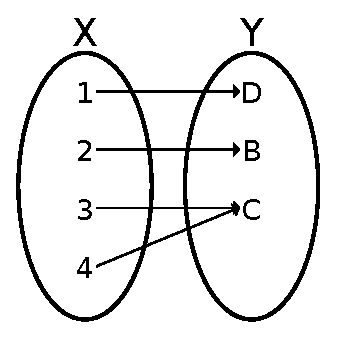
\includegraphics[height=2cm]{surjection.eps}}
    \hspace{0.1\textwidth}
    \subfloat[\(h^\prime\colon X\to 
    Y\)]{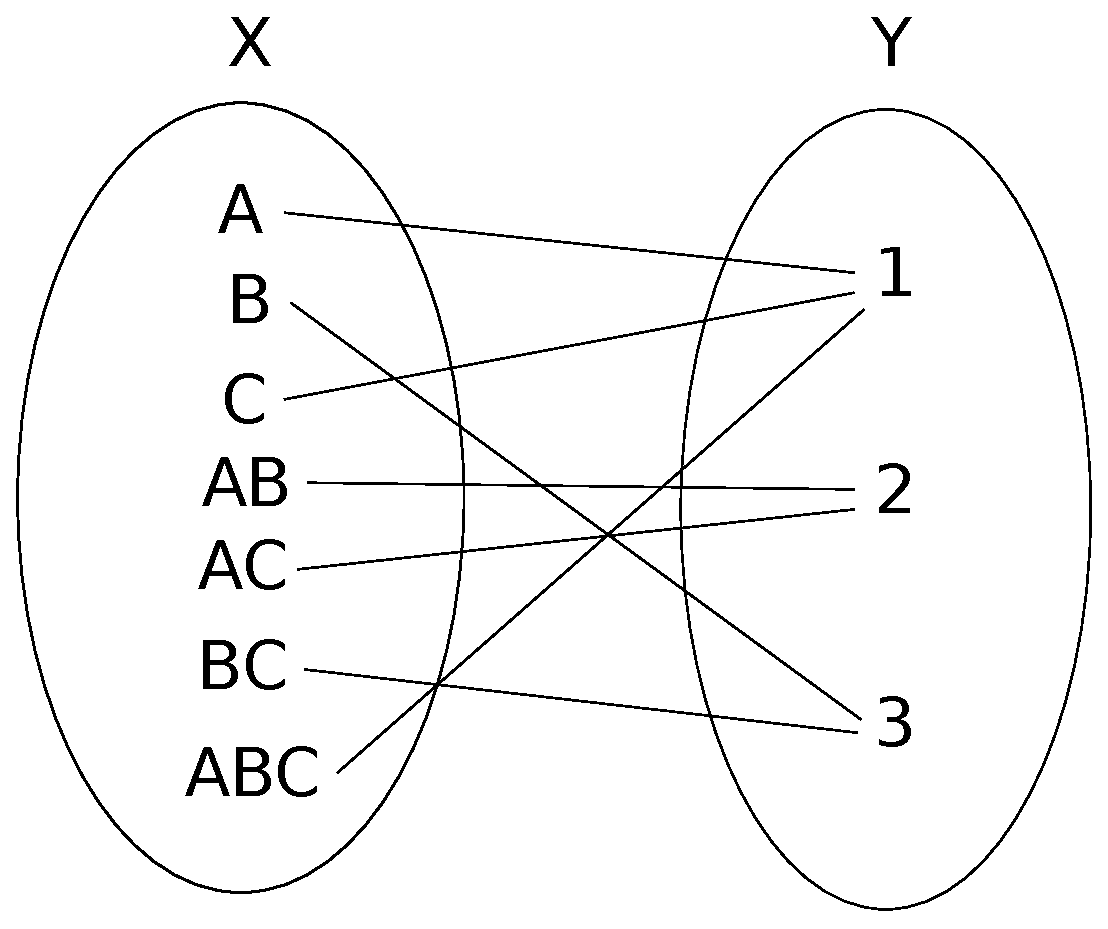
\includegraphics[height=2cm]{hashfunc.eps}}
    \caption{Två icke-injektiva surjektiva funktioner \(h\) respektive 
    \(h^\prime\).}
  \end{figure}
\end{frame}

\begin{frame}{\insertsubsectionhead}
  \begin{itemize}
    \item Finns många olika hashfunktioner:
      \begin{itemize}
        \item MD5,
        \item SHA1,
        \item SHA256,
        \item SHA512.
      \end{itemize}

    \item Tillämpningsområdet är stort:
      \begin{itemize}
        \item verifiera integritet hos filer,
        \item snabb sökning i datastrukturer,
        \item digitala signaturer,
        \item skydda lösenord.
      \end{itemize}

  \end{itemize}
\end{frame}

\subsection{Formell behandling av hashfunktioner}

\begin{frame}{\insertsubsectionhead}
  \begin{definition}
    En \emph{hashfamilj} är en tupel \((\X, \Y, \K, \H)\), där
    \begin{itemize}
      \item \(\X\) är mängden av möjliga \emph{meddelanden}.

      \item \(\Y\) är en ändlig mängd av möjliga \emph{meddelandesammandrag}.

      \item \(\K\) är en ändlig mängd av möjliga nycklar.

      \item För varje nyckel \(k\in \K\) finns en hashfunktion \(h_k\in \H\) 
        sådan att \(h_k\colon \X\to \Y\).

    \end{itemize}
  \end{definition}
\end{frame}

\begin{frame}{\insertsubsectionhead}
  \begin{itemize}
    \item \(\X\) kan vara ändlig eller oändlig, men alltid \(|\X|\geq |\Y|\).

    \item Vissa hashfunktioner saknar nycklar, då är \(|\K| = 1\).

    \item Låt \(\Y^{\X}\) beteckna mängden av alla funktioner från \(\X\) till 
      \(\Y\), då är \(|\Y^{\X}| = |\Y|^{|\X|}\).

  \end{itemize}
\end{frame}

\begin{frame}{\insertsubsectionhead}{\emph{Preimage resistant} eller 
  \emph{one-way}}
  \begin{block}{Inversa bilden (\emph{preimage})}
    \begin{enumerate}
      \item Given hashfunktionen \(h\colon \X\to \Y\) och element \(y\in \Y\).
      \item Hitta \(x\in \X\) sådant att \(h(x) = y\).
    \end{enumerate}
  \end{block}
\end{frame}

\begin{frame}{\insertsubsectionhead}{\emph{Second preimage resistant}}
  \begin{block}{Andra inversa förbilden (\emph{second preimage})}
    \begin{enumerate}
      \item Given hashfunktionen \(h\colon \X\to \Y\) och element \(x\in \X\).
      \item Hitta \(x^\prime\in \X\) sådant att \(x^\prime\neq x\) och 
        \(h(x^\prime) = h(x)\).
    \end{enumerate}
  \end{block}
\end{frame}

\begin{frame}{\insertsubsectionhead}{\emph{Collision resistant}}
  \begin{block}{Kollision}
    \begin{enumerate}
      \item Given hashfunktionen \(h\colon \X\to \Y\).
      \item Hitta \(x, x^\prime\in \X\) sådana att \(x^\prime\neq x\) och 
        \(h(x^\prime) = h(x)\).
    \end{enumerate}
  \end{block}
\end{frame}

\begin{frame}{\insertsubsectionhead}{Random Oracle Model}
  \begin{itemize}
    \item Idealisering av en hashfunktion.

    \item Kan liknas vid ett orakel som ger slumpmässiga svar på frågor.

    \item Men vid upprepningar ska samma svar ges.

    \item En funktion \(h\in \Y^{\X}\) väljs slumpmässigt, vi får enbart ställa 
      frågor som ''vad är \(h(x)\)?''

    \item Innan vi ställer frågan \(h(x)\) vet vi ingenting om \(h\).

    \item Efter att vi ställt frågan \(h(x)\) och erhållit svaret \(y\), då vet 
      vi enbart att \(h(x) = y\).

  \end{itemize}
\end{frame}

\begin{frame}{\insertsubsectionhead}
  \begin{itemize}
    \item Det går att visa att om man kan hitta en andra invers avbildning, då 
      kan man hitta en kollision.

    \item Det går även att visa att om man kan hitta en invers avbildning, då 
      kan man hitta en kollision.

    \item Följaktligen, om en hashfunktion är \emph{collision resistant}, då är 
      den även \emph{preimage} och \emph{second preimage resistant}.

  \end{itemize}
\end{frame}

\begin{frame}{\insertsubsectionhead}
  \begin{theorem}[Oberoendesatsen]
    Antag att \(h\in \Y^{\X}\) väljs slumpmässigt.
    Låt \(\X_0\subseteq \X\).
    Antag att värdet \(h(x)\) bestämts genom att fråga oraklet om och endast om 
    \(x\in \X_0\).
    Då gäller att \[\Pr(h(x) = y) = \frac{1}{|\Y|}\] för alla \(x\in \X 
    \setminus \X_0\) och alla \(y\in \Y\).
  \end{theorem}
\end{frame}

\begin{frame}{\insertsubsectionhead}
  % XXX fix bug which does not translate pseudocode
  \begin{algorithm}{Hitta invers avbild}
    \begin{algorithmic}
      \Require{\(h\in \Y^{\X}, y\in \Y, Q\in \N\)}
      \Ensure{\(x\) sådant att \(h(x) = y\)}
      \Statex
      \State Välj någon mängd \(\X_0\subseteq \X\) sådan att \(|\X_0| = Q\).
      \ForAll{\(x\in \X_0\)}
        \If{\(h(x) = y\)}
          \State \Return \(x\)
        \EndIf
      \EndFor
      \State \Return misslyckande
    \end{algorithmic}
  \end{algorithm}
\end{frame}

\begin{frame}{\insertsubsectionhead}
  \begin{theorem}
    För någon mängd \(\X_0\subseteq \X\) med \(|\X_0| = Q\) är sannolikheten 
    \(\epsilon\) att algoritmen för att finna en inverterad avbildning lyckas 
    \(\epsilon = 1 - \left(1 - \frac{1}{|\Y|}\right)^Q\).
  \end{theorem}
\end{frame}

%\begin{frame}{\insertsubsectionhead}
%  \begin{proof}
%    Fixera \(y\in \Y\).
%    Låt \(\X_0 = \{x_1, \ldots, x_Q\}\) och låt \(E_i\) beteckna händelsen att 
%    \(h(x_i) = y\).
%    Det följer från oberoendesatsen att \(E_i\) är oberoende händelser och att 
%    \(\Pr(E_i) = \frac{1}{|\Y|}\) för \(1\leq i\leq Q\).
%    Då får vi
%    \begin{align*}
%      \Pr(E_1\lor\cdots\lor E_Q) = 1 - \left(1 - \frac{1}{|\Y|}\right)^Q.
%    \end{align*}
%    Då sannolikheten \(\epsilon\) är oberoende av \(y\) och konstant, då måste 
%    sannolikheten vara densamma för alla \(y\in \Y\) sammantaget.
%  \end{proof}
%\end{frame}

\begin{frame}{\insertsubsectionhead}
  % XXX fix bug which does not translate pseudocode
  \begin{algorithm}{Hitta kollision}
    \begin{algorithmic}
      \Require{\(h\in \Y^{\X}, Q\in \N\)}
      \Ensure{\(x, x^\prime\in \X\) sådana att \(x\neq x^\prime, h(x) 
      = h(x^\prime)\)}
      \Statex
      \State Välj någon mängd \(\X_0\subseteq \X\) sådan att \(|\X_0| = Q\).
      \ForAll{\(x\in \X\)}
        \State Låt \(y_x = h(x)\).
      \EndFor
      \If{\(y_x = y_{x^\prime}\) för något \(x\neq x^\prime\)}
        \State \Return \((x, x^\prime)\)
      \EndIf
      \State \Return misslyckande
    \end{algorithmic}
  \end{algorithm}
\end{frame}

\begin{frame}{\insertsubsectionhead}
  \begin{theorem}
    För någon mängd \(\X_0\subseteq \X\) med \(|\X_0| = Q\) är sannolikheten 
    \(\epsilon\) för att kollisionsalgoritmen lyckas följande:
    \begin{align*}
      \epsilon = 1 - \left(\frac{|\Y|-1}{|Y|}\right)
        \left(\frac{|\Y|-2}{|\Y|}\right) \cdots
        \left(\frac{|\Y|-Q+1}{|\Y|}\right).
    \end{align*}
  \end{theorem}
\end{frame}

%\begin{frame}{\insertsubsectionhead}
%  \begin{proof}
%    \small
%    Låt \(\X_0 = \{x_1, \ldots, x_Q\}\).
%    För \(1\leq i\leq Q\), låt \(E_i\) beteckna händelsen
%    \begin{align*}
%      h(x_i)\notin \{h(x_1), \ldots, h(x_{i-1})\}.
%    \end{align*}
%    Det är klart att \(\Pr(E_1) = 1\), då \(h(x_1)\notin \emptyset\).
%    Vi får genom induktion från oberoendesatsen att
%    \begin{align*}
%      \Pr(E_i\mid E_1\land E_2\land \cdots\land E_{i-1}) = 1 - \frac{i-1}{|\Y|} 
%      = \frac{|\Y|-i+1}{|\Y|},
%    \end{align*}
%    för \(2\leq i\leq Q\).
%    Då har vi att
%    \begin{align*}
%      \Pr(E_1\land \cdots\land E_Q) = \left(\frac{|\Y|}{|\Y|}\right)
%        \left(\frac{|\Y|-1}{|Y|}\right)\cdots
%        \left(\frac{|\Y|-Q+1}{|\Y|}\right).
%    \end{align*}
%    Följaktligen blir sannolikheten för minst en kollision \(1 - \Pr(E_1\land 
%    \cdots\land E_Q)\).
%  \end{proof}
%\end{frame}

\begin{frame}{\insertsubsectionhead}
  \begin{itemize}
    \item Vi hade att sannolikheten för ingen kollision är 
      \(\prod_{i=1}^{Q-1}(1 - 1/|\Y|)\).

    \item För små \(x\) gäller att \(1 - x\approx e^{-x}\).

    \item Då får vi \[\prod_{i=1}^{Q-1}(1-1/|\Y|)\approx \prod_{i=1}^{Q-1} 
      e^{-i/|\Y|} = e^{\sum_{i=1}^{Q-1} i/|\Y|}.\]

    \item Följaktligen gäller \(e^{\sum_{i=1}^{Q-1} i/|\Y|}\approx 
      1-\epsilon\).

    \item Med lite omskrivningar får vi \(Q\approx 
      \sqrt{2|\Y|\log\frac{1}{1-\epsilon}}\).

    \item För \(\epsilon = 1/2\) får vi då \(Q\approx 1.17\sqrt{|\Y|}\).

  \end{itemize}
\end{frame}

\begin{frame}{\insertsubsectionhead}
  \begin{itemize}
    \item Detta kallas födelsedagsparadoxen.

    \item Detta betyder att om \(|\Y| = 365\), då är den \unit{50}{\%} 
      sannolikhet att kollisionsalgoritmen finner en kollision då \(Q = 23\).

    \item Om en fingeravtrycksläsare lagrar fingeravtryck som 20 bitar långa 
      bitsträngar, då är det \unit{50}{\%} sannolikhet att två personer kan 
      identifiera sig som varandra vid 1000 användare.

    \item Vi kan finna kollisioner med \unit{50}{\%} sannolikhet för en 
      hashfunktion som har 256 bitars meddelandesammandrag med \(2^{128}\) 
      gissningar.

  \end{itemize}
\end{frame}

\begin{frame}{\insertsubsectionhead}
  \begin{description}
    \item[MD5] Fullständigt knäckt; kan finna godtyckliga kollisioner, snabb 
      att beräkna \citep[se][]{Lucks2005hc}.

    \item[SHA1] Finns attacker som antyder att det går att finna kollisioner 
      med \(Q = 2^{69}\), borde vara \(Q = 2^{80}\).

    \item[SHA256] Inga attacker som är märkbart lägre än \(Q = 2^{128}\).

    \item[SHA512] Inga attacker som är märkbart lägre än \(Q = 2^{256}\).

  \end{description}
\end{frame}


\section{Meddelandeautentisering}

\subsection{Message Authentication Code (MAC)}

\begin{frame}{\insertsubsectionhead}
  \begin{itemize}
    \item Vi har sett att både symmetrisk och asymmetrisk kryptering kan 
      användas för att signera kod.

    \item Dock uppstår problem om vi använder exempelvis ECB som mode of 
      operation.
      \begin{itemize}
        \item Byt ordning på blocken.
        \item Ta bort vissa block.
      \end{itemize}

    \item För detta ändamål skapar vi MAC.

  \end{itemize}
\end{frame}

\subsection{Hashfunktionsbaserade MAC}

\begin{frame}{\insertsubsectionhead}
  \begin{figure}
    \includegraphics[height=0.7\textheight]{mac.eps}
    \caption{En översikt av en enkel MAC.
      Bild: \citep{Stallings2013nse}.}
  \end{figure}
\end{frame}

\begin{frame}{\insertsubsectionhead}
  \begin{figure}
    \includegraphics[height=0.7\textheight]{mac-hash.eps}
    \caption{Exempel på olika former av MAC.
      Bild: \citep{Stallings2013nse}.}
  \end{figure}
\end{frame}

\begin{frame}{\insertsubsectionhead}
  \begin{figure}
    \includegraphics[height=0.7\textheight]{hmac.eps}
    \caption{Hashbaserad MAC kallad HMAC, \(\hmac(K, M) = h[ (K^+\xor opad) 
      \concat h[ (K^+\xor ipad) \concat M]]\).
      Bild: \citep{Stallings2013nse}.}
  \end{figure}
\end{frame}

\subsection{MAC baserade på blockchiffer}

\begin{frame}{\insertsubsectionhead}
  \begin{figure}
    \centering
    \includegraphics[height=0.7\textheight]{cmac.eps}
    \caption{En schematisk översikt av CMAC.
      Bild: \citep{Stallings2013nse}.}
  \end{figure}
\end{frame}

\subsection{Chiffer med autentisering}

\begin{frame}{\insertsubsectionhead}
  \begin{itemize}
    \item Counter with Cipher Block Chaining Message Authentication Code (CCM).

    \item Är ett mode of operation för kryptering med autentisering.

  \end{itemize}
\end{frame}

\begin{frame}{\insertsubsectionhead}
  \begin{figure}
    \centering
    \includegraphics[height=0.7\textheight]{ccm.eps}
    \caption{En schematisk översikt av CCM.
      Bild: \citep{Stallings2013nse}.}
  \end{figure}
\end{frame}


% XXX add section on BankID
%\section{BankID}
%
%\subsection{Uppbyggnad}
%\begin{frame}{\insertsubsectionhead}
%\end{frame}


%\section{Nyckelutbyte}
%
%\subsection{Principerna för nyckelutbyte}
%\begin{frame}{\insertsubsectionhead}
%\end{frame}
%
%\subsection{Diffie--Hellman nyckelutbyte}
%\begin{frame}{\insertsubsectionhead}
%\end{frame}


%%%%%%%%%%%%%%%%%%%%%%

\begin{frame}[allowframebreaks]{Referenser}
	\small
  \printbibliography
\end{frame}

\end{document}
